\documentclass[11pt]{beamer}
\usetheme{Warsaw}
\usepackage[utf8]{inputenc}
\usepackage{amsmath}
\usepackage{amsfonts}
\usepackage{amssymb}
\author{Maël FRANCESCHETTI\\Daoud KADOCH\\Fabien MANSON\\Nicolas CASTANET}
%\graphicspath{images\}
\logo{
\includegraphics[height=0.8cm]{logo_sorbonne.png}}
\title{Projet 3i013}
%\setbeamercovered{transparent} 
%\setbeamertemplate{navigation symbols}{} 
\institute{Sorbonne Université} 
\date{Lundi 25 Février 2019} 
%\subject{} 
\usepackage{pifont}% http://ctan.org/pkg/pifont
\begin{document}

\begin{frame}
\titlepage
\end{frame}

\section{Sommaire}
\begin{frame}
\frametitle{Sommaire}
\tableofcontents[sections={1-8}]
\end{frame}

%___________________________________________

%\section{Problématique et Objectifs}
%\begin{frame}
%\frametitle{Problématique et Objectifs}
%\begin{center}
%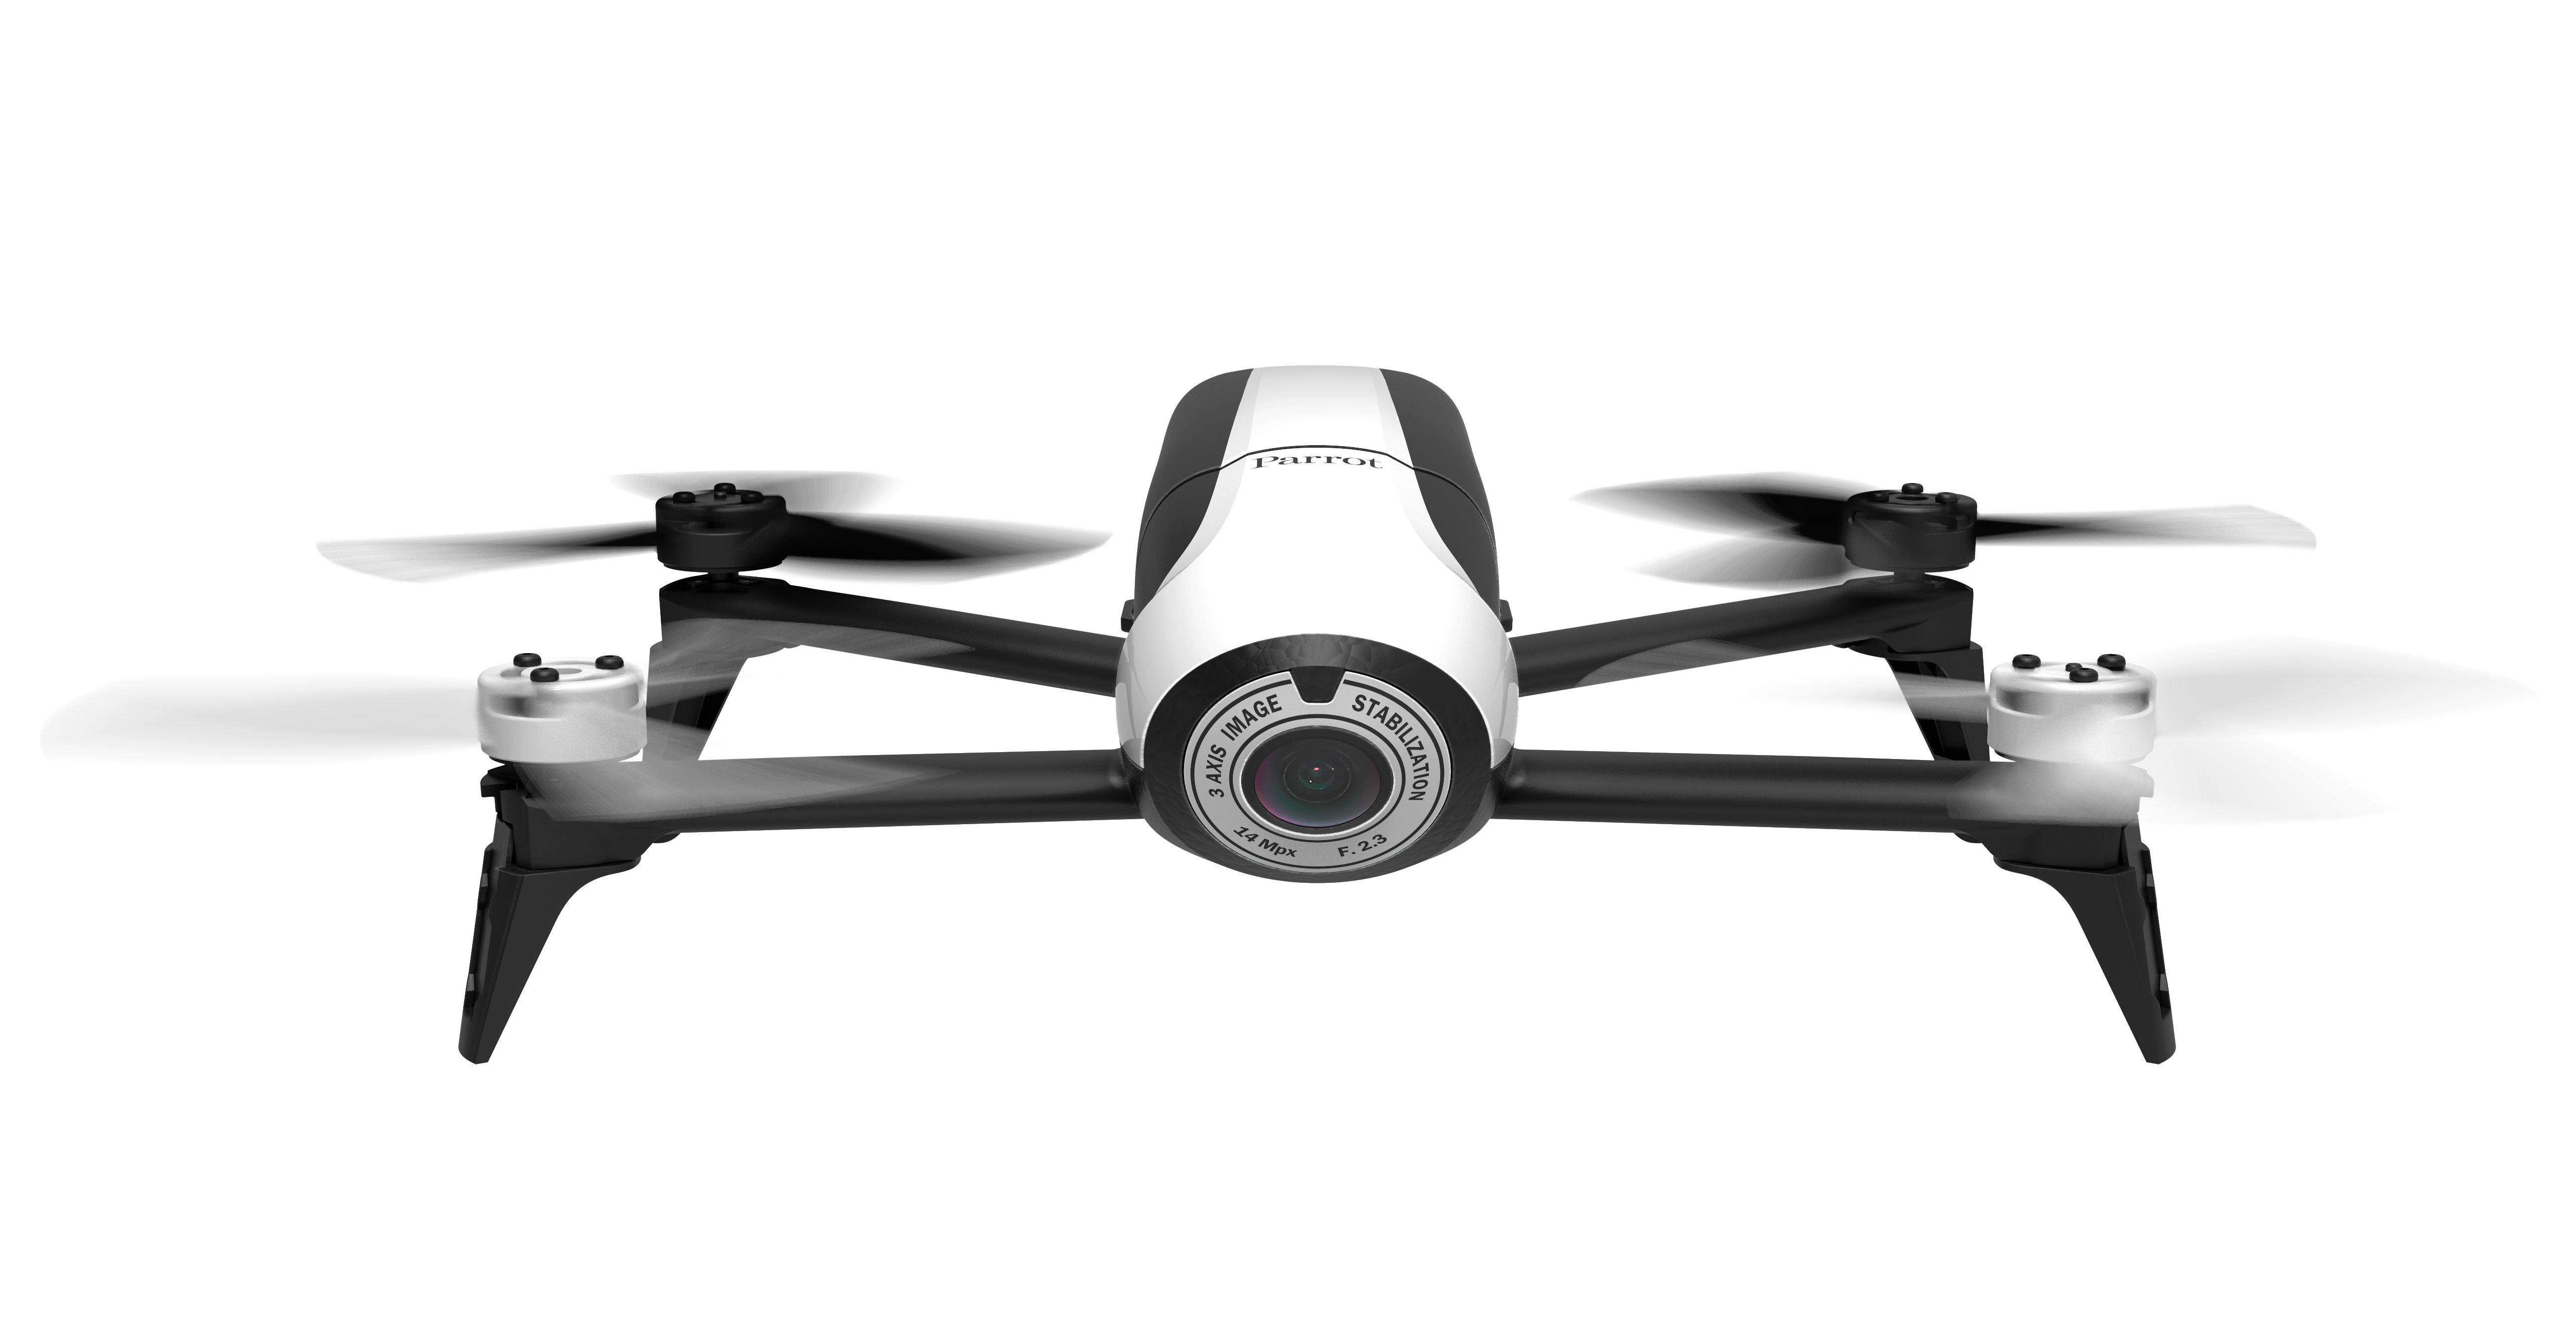
\includegraphics[height=4cm]{bebop_face.jpg}
%\end{center}
%\end{frame}

%___________________________________________

\section{Les attentes du client}
\begin{frame}
\frametitle{Les attentes du client}
\begin{itemize}
\item Programmer des rondes de surveillances : suivre un plan de vol
\item Interface Graphique : 
\begin{itemize}
\item Ergonomique (ex : tracé plan de vol tactile)
\item Intuitive 
\item Jolie (dans la mesure du possible)
\end{itemize}
\item Retour vidéo :
\begin{itemize}
\item Bonne résolution
\item Fluidité élevée
\item Latence réduite (quelques millisecondes)
\end{itemize}
\item Sécurité du vol :
\begin{itemize}
\item Bloquer les connexions externes entrantes
\item Fonction d'arrêt d'urgence
\end{itemize}

\end{itemize}
%\begin{center}
%
\includegraphics[height=5cm]{point.png}
%\end{center}
\end{frame}

%___________________________________________

\section{Le matériel à disposition}
\begin{frame}
\frametitle{Le matériel}
\begin{center}
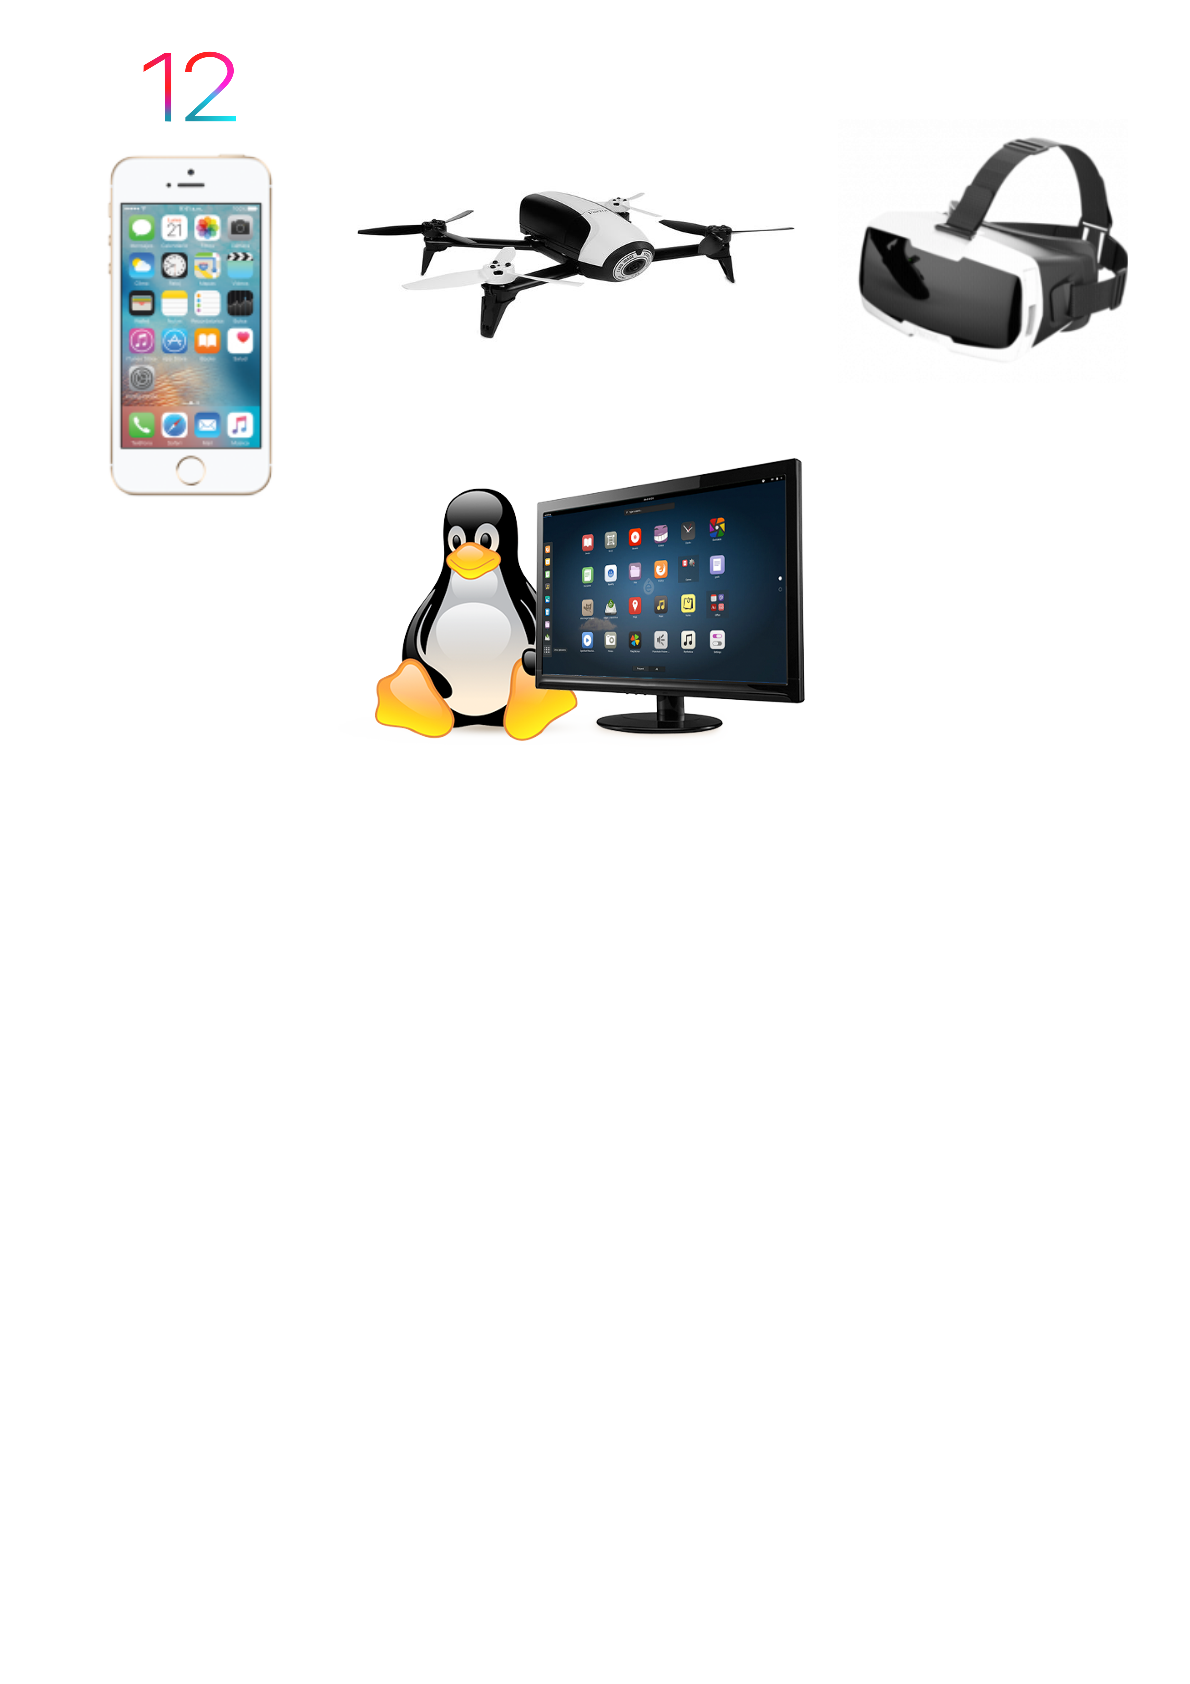
\includegraphics[height=13cm]{acteurs.png}
\end{center}
\end{frame}

%___________________________________________

\section{Première solution : Drone + PC + iPod}
\begin{frame}
\frametitle{Drone + PC + iPod}
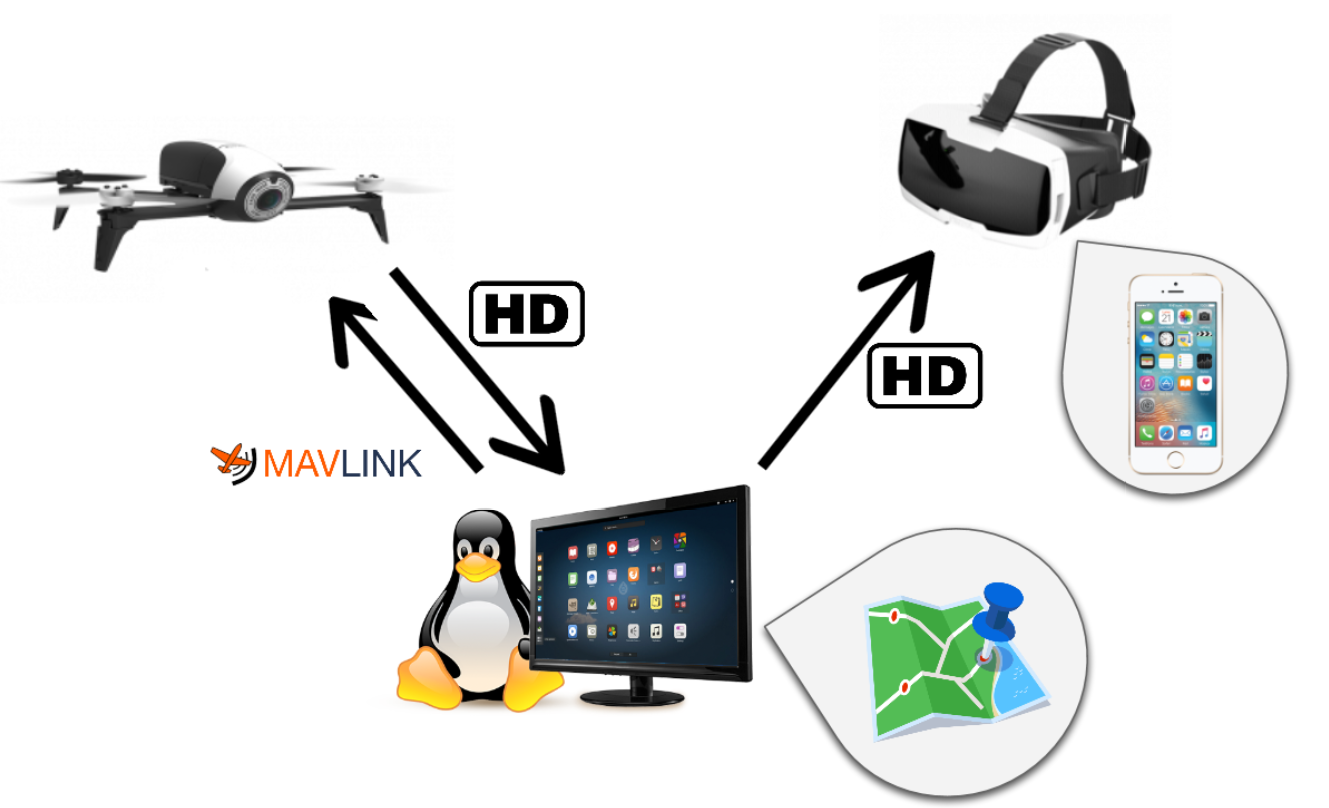
\includegraphics[height=7cm]{schemaPC.png}
\end{frame}

%___________________________________________

\subsection{Avantages}
\begin{frame}
\frametitle{Avantages}

\begin{itemize}
\item Puissance de calcul de l'ordinateur bien supérieure à celle d'un ipod%\ding{52}
    
\item Split screen de l'iPod pour le FPV %\ding{52}
\item Contrôle de l'arrêt d'urgence plus accessible
\end{itemize}
\end{frame}

%___________________________________________

\subsection{Inconvénients}
\begin{frame}
\frametitle{Inconvénients}
\begin{itemize}

\item Double connexion wifi : Drone vers PC, PC vers iPod %\ding{54}
    
\item Double redirection du flux vidéo : Drone vers PC vers iPod %\ding{54}

\item Communication Linux/IOS complexe %\ding{54}

\item Deux applications à développer %\ding{54}

\item Ergonomie d'utilisation : vol sans PC impossible%\ding{54}

\item Beaucoup de bibliothèques à assimiler %\ding{54}
\end{itemize}
\end{frame}

%___________________________________________

\section{Deuxième solution : se passer du Pc}
\begin{frame}
\frametitle{Drone + iPod}
\begin{center}
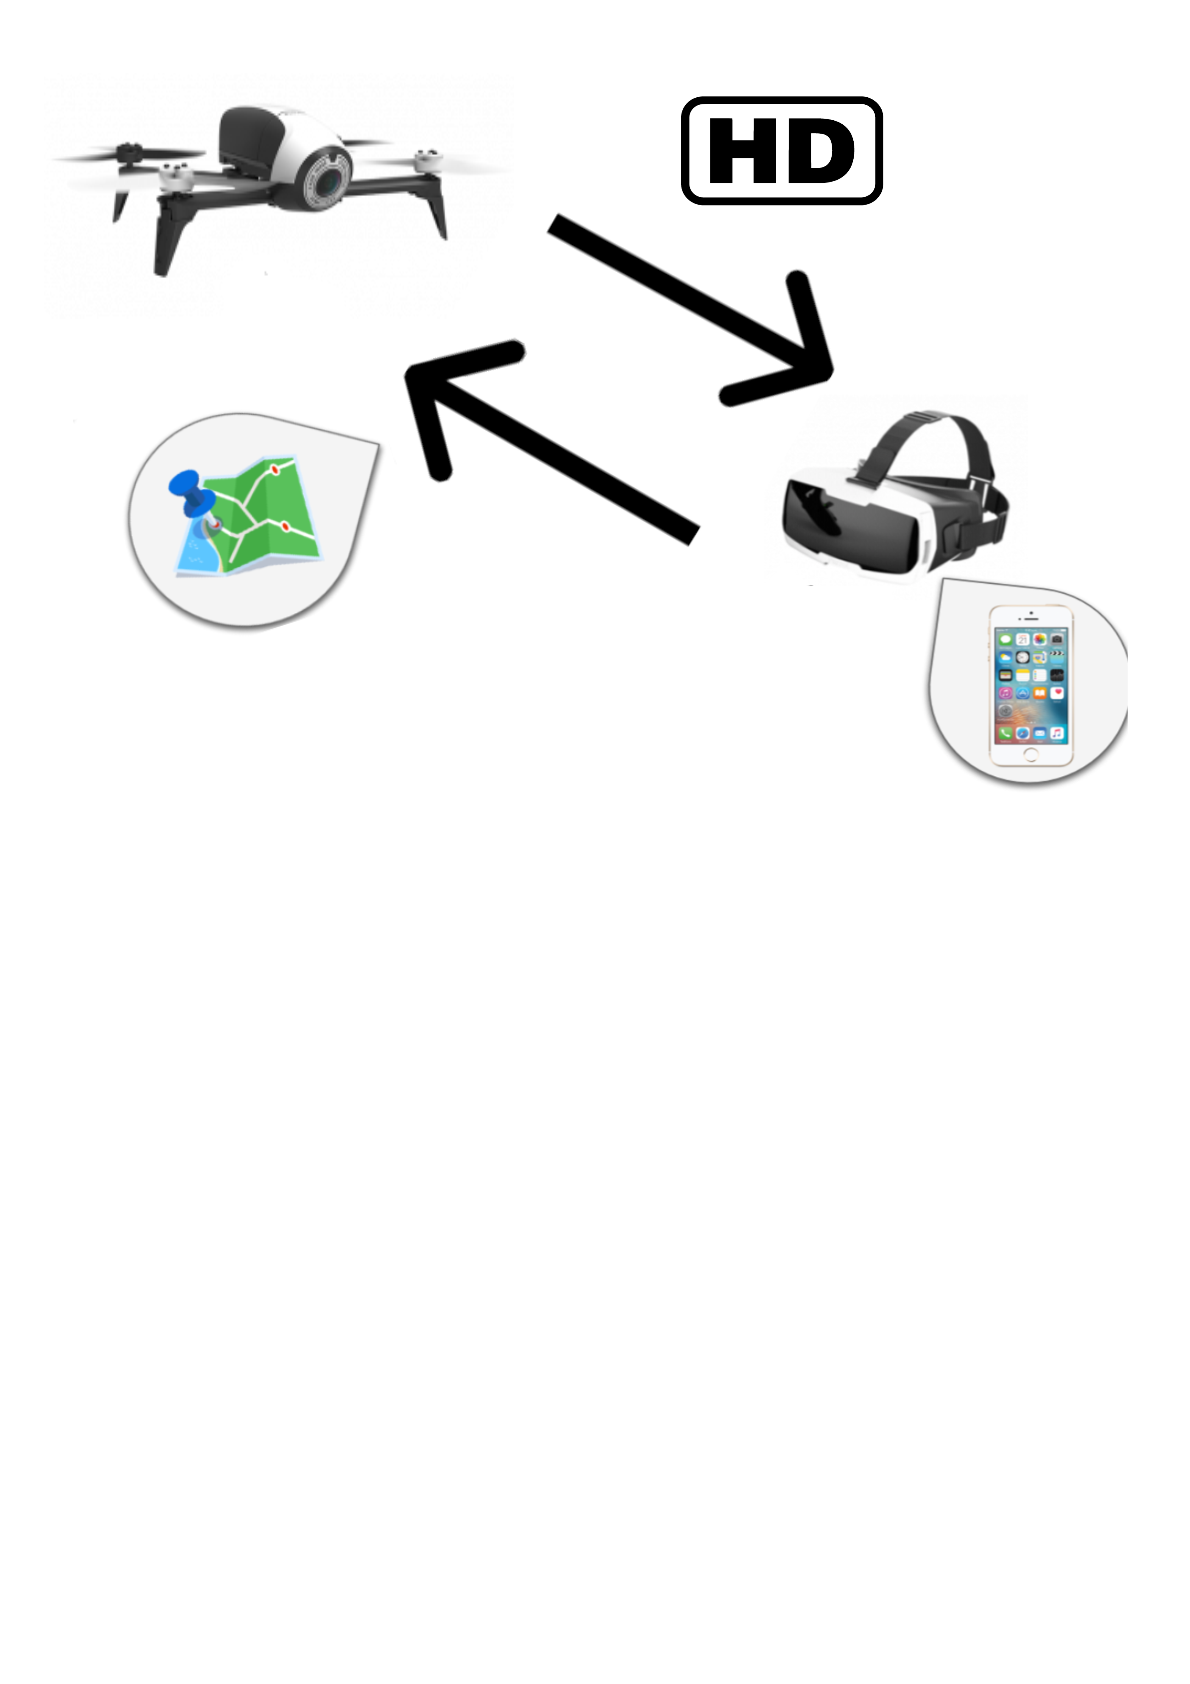
\includegraphics[height=13cm]{drone+ipod.png}
\end{center}
\end{frame}

%___________________________________________

\subsection{Avantages}
\begin{frame}
\frametitle{Avantages}
\begin{itemize}
    \item Un seul langage de programmation : Objective-C %\ding{52}
    
    \item Une seule application à développer %\ding{52}
    
    \item pas de double redirection du flux vidéo %\ding{52}
    
    \item Meilleure ergonomie pour l'utilisateur : interface tactile%\ding{52}
  \end{itemize}
\end{frame}

%___________________________________________

\subsection{Inconvénients}
\begin{frame}
\frametitle{Inconvénients}

\begin{itemize}
    \item Contrôle d'urgence du drone inaccessible car l'iPod est dans le casque%\ding{54}
    
    \item Traitement du flux vidéo lourd pour un terminal mobile%\ding{54}
    \item Portée de la connexion wifi limitée : perte du signal vidéo 
    \item Environnement de développement Apple totalement inconnu
        
  \end{itemize}
\end{frame}

%___________________________________________

\section{Conclusion}
\begin{frame}
\frametitle{Conclusion}
\begin{center}
\hspace{-0.5cm}
\begin{tabular}{|c|c|c|}
\hline
 & Drone + Pc + iPod & Drone + iPod \\
 \hline
 Puissance de calcul (vidéo)& + & - \\
 \hline
 Ergonomie interface & - & +\\
 \hline
 Accès contrôle d'urgence & + & -\\
 \hline
 Portée Communication & + & -\\
 \hline
 Simplicité connexion Wifi & - & +\\
 \hline
 Complexité de développement & - & +\\
 \hline
 
\end{tabular}
\end{center}
%\begin{center}
%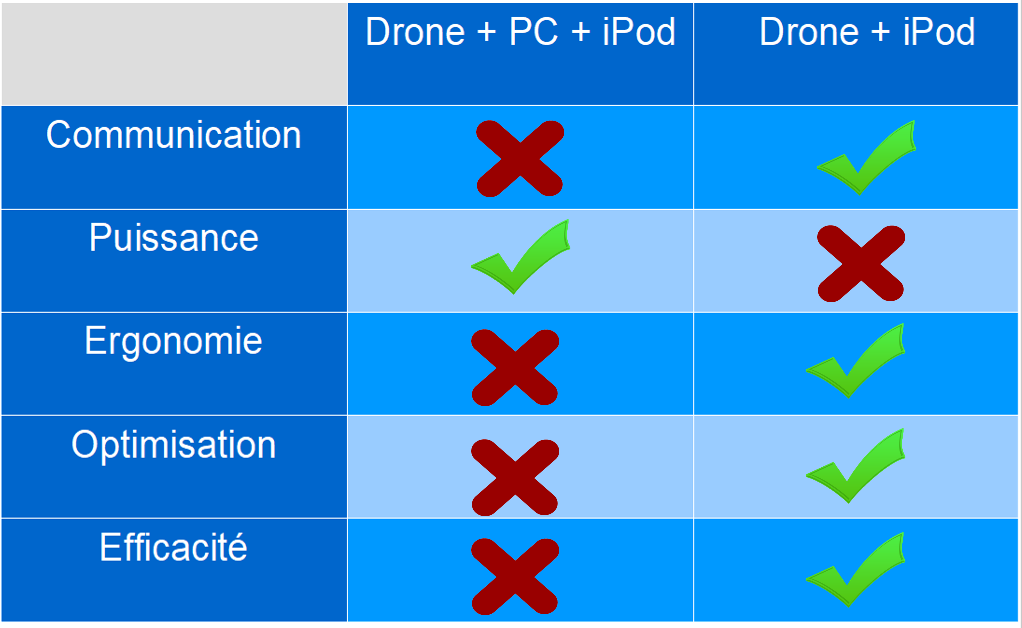
\includegraphics[height=5cm]{tableau.png}
%\end{center}
\end{frame}

%___________________________________________

\end{document}

%___________________________________________